\documentclass[12pt]{article}
\usepackage{tikz}
\usepackage{pgfplots}
\usepackage[utf8]{inputenc}
\usepackage[english]{babel}
\usepackage{xcolor}
\usepackage{textcomp}
\usepackage[hyphens,spaces,obeyspaces]{url}
\usepackage{listings}
\lstset{language=C++,
	basicstyle=\ttfamily,
	keywordstyle=\color{blue}\ttfamily,
	stringstyle=\color{red}\ttfamily,
	commentstyle=\color{green}\ttfamily,
	morecomment=[l][\color{magenta}]{\#}
}

\usepackage{amsmath,amsthm,amssymb,amsfonts}
\usepackage{booktabs}
\usepackage{array}
\usepackage{fancyhdr}
\usepackage[a4paper, margin=1in]{geometry}
\usepackage{multicol}
\usepackage{enumerate}
\usepackage{graphicx}
\usepackage{subcaption}
\graphicspath{ {./images/} }
\usepackage[super]{nth}

\newtheorem{theorem}{Theorem}
\newtheorem{corollary}{Corollary}[theorem]
\newtheorem{definition}{Definition}
\newtheorem{lemma}{Lemma}
\theoremstyle{remark}
\newtheorem*{remark}{Remark}

\newcommand{\N}{\mathbb{N}}
\newcommand{\Z}{\mathbb{Z}}
\newcommand{\R}{\mathbb{R}}
\newcommand{\mat}[1]{\mathbf{#1}}
\newcommand{\norm}[1]{\left\lVert#1\right\rVert}
\newcommand{\PreserveBackslash}[1]{\let\temp=\\#1\let\\=\temp}
\newcolumntype{C}[1]{>{\PreserveBackslash\centering}p{#1}}
\newcolumntype{R}[1]{>{\PreserveBackslash\raggedleft}p{#1}}
\newcolumntype{L}[1]{>{\PreserveBackslash\raggedright}p{#1}}

\pagestyle{fancy}
\fancyhf{}
\rhead{TSE, Ho Nam}
\chead{Project \#2}
\lhead{MATH4828B}
\cfoot{\thepage}
\title{
  {\large MATH4828B Machine Learning for Natural Language Processing}\\
  \textbf{\large Project 2 -- Sentiment Analysis}\\
  \textbf{Report}
  }
\author{ 
  \begin{tabular}{R{0.4\textwidth}L{0.4\textwidth}}
    \textbf{Name:} & TSE, Ho Nam \\
    \textbf{Student ID:} & 20423612 \\
    \textbf{Kaggle Team Name:} & 20423612 \\
    \textbf{Kaggle Username:} & Peter Tse (\texttt{mcreng}) \\
    \textbf{Ranking (Score):} & \nth{7} (0.64506)
  \end{tabular}
 }
  
\date{}

\begin{document}
\maketitle\thispagestyle{fancy}
\begin{abstract}
	This report discusses the methodology used to train the neural network used in participat\-ing the Kaggle competition. In short, \texttt{Jupyter Notebook} was used to run the codes and they were mainly written with help of the libraries \texttt{numpy}, \texttt{sklearn} and \texttt{nltk}. Before the data were fed into the neural network, preprocessing such as tokenization, words removal, \(n\)-grams and tfidf were use. Word lemmatization was also attempted but it did not increase the accuracy sufficiently and it cost much longer processing time so it was no longer used. The neural network used was Multilayer Layer Perceptron with Xaiver initialization, cross-entropy loss and Adam update rule. Its regularization coefficient, hidden layer size and activation function were considered as hyperparameters and \(k\)-fold cross validation was used to consider which combination of the hyperparameters are the best. At last, the neural network with hidden size \((50, 50,)\), regularization coefficient of \(\sim0.03\) and logistic activation function was used to predict the test case. This network scored 0.64506 in the competition, ranking seventh.
\end{abstract}

\section{Preprocessing}

\subsection{Tokenization}
Before any preprocessing, the documents are read and tokenized through \texttt{nltk} tokenizer.

\subsection{Stop Word Removal}
As the documents are read, some stop words are removed from the documents. These stop words contain commonly used words that carry insignificant meanings in the document. They are a composition of \texttt{nltk} stop words and a self-made list of

\begin{lstlisting}[language=python]
  ["'d", "'ll", "'re", "'s", "'ve", "`'", "could", \
  "might", "must", "n't", "need", "sha", "wo", "would"].
\end{lstlisting}

These additional stop words are used because the \texttt{nltk} stop words could not remove these words and these words appear to be insignificant in meaning as well.

I also added a check of \lstinline[language=python]{len(word) > 1} which remove all words with length of 1. These words are not meaningful and sometimes might be created through a typo.

\begin{quote}
	we didnt eat expensive.the staff ok. just not special 140 \textbf{e} excluding tax no breakfast. confirmation said internet facilities none.
\end{quote}

\subsection{Punctuation Removal}
The punctuation marks in the documents are removed since they do not give much insights towards the sentiment analysis. They are removed by considering

\noindent\hspace{0.35\textwidth}\lstinline[language=python]{list(string.punctuation).}

\subsection{Word Lowercase}
Cases seems to be not useful in the document since by briefing looking at the document, the words are mainly in lowercase.
\begin{quote}
	cozy stay rainy city. husband spent 7 nights \textbf{monaco} early \textbf{january} 2008. business trip chance come ride. we booked \textbf{monte carlo} suite proved comfort\-able longish stay.
\end{quote}
The bolded words in the quote above should be in uppercase when written in standard English, but since they are not, it seems we cannot gather useful information by looking at cases. Since it is not sure if there are some documents with words in uppercase, to prevent the same words in different cases being counted separately, all the words are set to lowercase.

\subsection{Number Removal}
It is suspected that this task is in fact about hotel reviews, that the documents given are the reviews, and the categorical outputs are the number of stars given in this review. It might be useful to look for numbers in the text since reviewers might put `Great hotel! 5 stars!' in the reviews and we hence can directly get the category corresponding to the review. However, there are too many other unrelated occurrences of numbers which makes it difficult to check whether the number is about the number of stars the reviewers give. Also, sometimes we have pieces of text like
\begin{quote}
	lawn mowers 5 a.m. given room golf course. woke 5 morning roar lawn mowers. 5 numerous fairways. wear tear rooms facilities obvious. beautiful old hotel \textbf{not 3 stars}. bring earplugs.
\end{quote}
which might fool the network that this review corresponds to 3 stars (which in fact corresponds to 1 star) if we consider the numbers. Therefore, numbers are removed to reduce the ambiguity caused by the presence of numbers. The removal of numbers is done by \lstinline[language=python]{word.isnumeric()}.

\subsection{Lemmatization}
Lemmatization is the process of change the word into its corresponding common base form, which is achieved by using morphological analysis of words. For example\footnote{Example adapted from Stanford NLP: \url{ https://nlp.stanford.edu/IR-book/html/htmledition/stemming-and-lemmatization-1.html}}, we have
\begin{center}
	\begin{tabular}{ccc}
		\toprule
		\textbf{Before} &                 & \textbf{After} \\\midrule
		the             & \(\rightarrow\) & the            \\\midrule
		boy's           & \(\rightarrow\) & boy            \\\midrule
		cars            & \(\rightarrow\) & car            \\\midrule
		are             & \(\rightarrow\) & be             \\\midrule
		different       & \(\rightarrow\) & differ         \\\midrule
		colors          & \(\rightarrow\) & color          \\\bottomrule
	\end{tabular}
\end{center}
This might help increase the accuracy since with lemmatization, words with same base form can be grouped together. This is achieved by using \lstinline[language=python]{WordNetLemmatizer} in the \texttt{nltk} library. Since this lemmatizer requires the part of speech tag of each word as well, we also use \lstinline[language=python]{nltk.pos_tag(tokens)}.

Lemmatization is \textbf{not} used in the final models though, since it requires a long time to compute, and the accuracy does not increase significantly after lemmatization.

\subsection{\(n\)-gram}
In our data preprocessing model, each word is captured separately which means phrases like \texttt{Hong Kong} cannot be captured. Therefore, apart from considering word by word, we also consider \(n\)-gram, which means we also consider contiguous sequence of \(n\) words in the documents as well. For example, a sentence of
\begin{quote}
	``I love Hong Kong."
\end{quote}
can have \(n\)-grams of following.
\begin{center}
	\begin{tabular}{cc}
		\toprule
		\(n\)-gram & Examples                     \\\midrule
		\(1\)-gram & I, love, Hong, Kong          \\\midrule
		\(2\)-gram & I love, love Hong, Hong Kong \\\midrule
		\(3\)-gram & I love Hong, love Hong Kong  \\\midrule
		\(4\)-gram & I love Hong Kong             \\\bottomrule
	\end{tabular}
\end{center}
In particular, our model uses \(n\)-grams with \(n=1\) to \(5\).

\subsection{Head/Tail Word Removal}
Consider the example in \(n\)-gram above, some phrases like ``love Hong'' does not make sense. Some phrases that appear rarely may also not contribute to the meaning of the documents. These can be regarded as the tail phrases and can be removed. In our model, we remove phrases that do not appear more than 3 times in total.

Some words may appear very often, for example in our dataset, \texttt{hotel} and \texttt{room} appear very frequently. They may also not help classifying the documents since they are ubiquitous. These words are regarded as head words and can also be removed. In our model, phrases that appear in more than 99.9\% of all documents are removed.

\subsection{TFIDF}
TFIDF is a weighting applied to a document-vocabulary matrix. Usually when as a word appears more often in a single document, this word might be important in that document so we might want to weigh it more. However, if a word appears frequently across all documents, this might mean this word is not useful in distinguishing the documents. Therefore, a weighting of the product of term frequency (tf) and inverse document frequency (idf) can be used to apply to the document-vocabulary matrix.

In our model, after processing all documents, the document-vocabulary matrix uses the following tf and idf functions.
\[
	\text{tf}(t, d) = f_{t,d}, \qquad \text{idf}(t) = 1,
\]
where \(f_{t,d}\) is the frequency of term \(t\) in document \(d\). This means we just use the number of occurrences of each word in each document as the entry of the data matrix. Other choices of idf were tried such as \[
	\text{idf}(t) = \log \frac{N}{n_t},
\]
where \(N\) is the number of documents and \(n_t\) is the number of document term \(t\) appears in, but they do not seem to give better results. One hypothesis is that the training data is skewed towards 5-star reviews which after applying idf, classifications with positive reviews might perform worse since the positive words are treated with less significance.

\begin{center}
	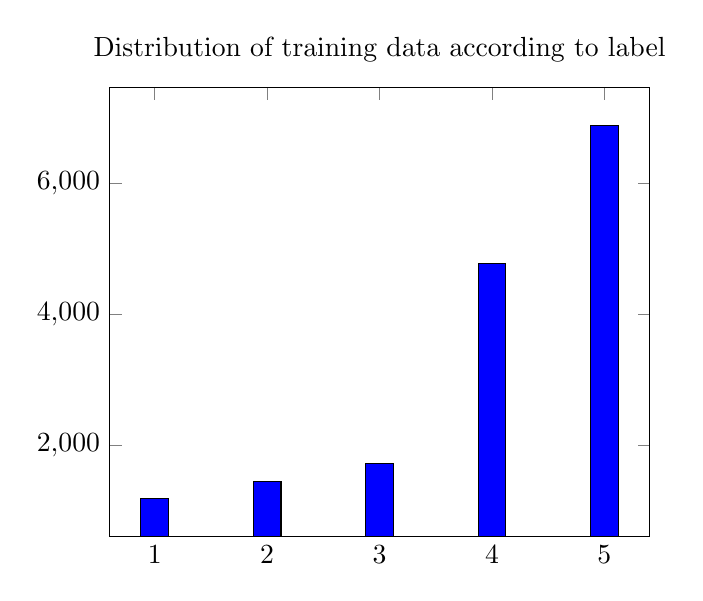
\begin{tikzpicture}
		\begin{axis}[
				symbolic x coords={1, 2, 3, 4, 5},
				xtick=data,
				title=Distribution of training data according to label
			]
			\addplot[ybar,fill=blue] coordinates {
					(1, 1179)
					(2, 1440)
					(3, 1716)
					(4, 4774)
					(5, 6891)
				};
		\end{axis}
	\end{tikzpicture}
\end{center}


\subsection{Saving Processed Data}
To avoid preprocessing the same set of data every time a model is trained, the preprocessed data are stored as \texttt{.npy} files, a compressed binary file for \texttt{numpy} arrays. It is achieved by \lstinline[language=python]{np.save(filename, obj)} where \texttt{filename} is the location to store the files and \texttt{obj} is the array to be stored.

\section{Neural Network}
After preprocessing the data, they are fed into a Multilayer Perceptron neural network initialized with uniform distribution with cross-entropy loss and Adam as update rule. Logistic activation function is used in the hidden layers and Softmax is used in the output layer in the final model.

\subsection{Multilayer Perceptron}
\begin{definition}
	A neuron can be considered as a function that takes \(n\) inputs, \(m\) outputs and an activation function \(\sigma: \R^m \to \R^m\) that has the structure
	\[
		\mat y = \sigma(\mat W \mat x + \mat b),
	\]
	where
	\(\begin{aligned}[t]
		 & \mat y \in \R^m            &  & \text{is the output,}        \\
		 & \mat W \in \R^{m \times n} &  & \text{is the weight matrix,} \\
		 & \mat b \in \R^m            &  & \text{is the bias, and}      \\
		 & \mat x \in \R^n            &  & \text{is the input}.
	\end{aligned}\)
\end{definition}
\begin{remark}
	This definition of neuron is actually a generalization of a perceptron, that a perceptron only takes in 1 input and gives out 1 output, and its activation function is defined.
\end{remark}
\noindent With the definition of a neuron, we can then define multilayer perceptron.
\begin{definition}
	Multilayer Perceptron (MLP) is a feed-forward network that consists of multiple layers: Input layer, Hidden layers and Output layer. Except the input layer, every layer has multiple neurons with nonlinear activation functions. Neurons in one layer take inputs from all neurons in their previous layer, and output to all neurons to their next layer.
\end{definition}
\begin{figure}[!h]\label{fig:mlp}
	\includegraphics[width=0.6\textwidth]{mlp}
	\centering
	\caption{Multilayer Perceptron Structure}
\end{figure}

This network usually outperforms other classifiers such as Na\"ive Bayes, Perceptron and Logistic Regression because MLP can handle data that is not linearly separable. This is because even the term \(\mat W \mat x + \mat b\) is a linear function, the activation function is not linear and thus, the network can model nonlinear functions. Figure~\ref{fig:nonlinear-dataset} shows experimental results of different classifiers on nonlinear dataset. Since it is generally not true that the training data is linearly separable, MLP is used in this case.

\begin{figure}[!h]
	\centering
	\begin{subfigure}[b]{0.4\textwidth}
		\includegraphics[width=\textwidth]{perceptron-nonlinear}
		\caption{Perceptron on Nonlinear Dataset}
		\label{fig:perceptron-nonlinear}
	\end{subfigure}
	\begin{subfigure}[b]{0.4\textwidth}
		\includegraphics[width=\textwidth]{mlp-nonlinear}
		\caption{MLP on Nonlinear Dataset}
		\label{fig:mlp-nonlinear}
	\end{subfigure}
	\caption{Classifers on Nonlinear Dataset\protect\footnotemark}\label{fig:nonlinear-dataset}
\end{figure}
\footnotetext{Images generated from Tensorflow Playground: \url{https://playground.tensorflow.org/}}

For each forward pass of the network, we have some input \(\mat x\) and it corresponds to a class of 1 to 5. As \(\mat x\) is passed through the network, we would expect the output vector has the highest value in the \(i\)-th entry where \(i\) is the corresponding class of \(\mat x\).

\subsection{Initialization}
Before training, the weights and biases of the neurons need to be initialized. In our model, the initialization suggested by Xaiver and Yoshua\footnote{\url{http://proceedings.mlr.press/v9/glorot10a/glorot10a.pdf}} is used for the weights and the biases are initialized as 0. Xaiver et al. suggests to initialize the weight \(W\) with \[
	W \sim U\left[-\sqrt{\frac{6}{n+m}}, \sqrt{\frac{6}{n+m}}\right],
\]
where \(n\) and \(m\) are the number of nodes in the previous and next layer respectively. The randomness is necessary since otherwise all neurons would have exactly the same behaviour. The weight is normalized by the number of nodes in neighbouring layers so that during back-propagation, the gradient would not explode or vanish over a deep network (since in each back-propagation step, the gradient w.r.t. the input is multiplied by the weight once).

\subsection{Activation Functions}
In the design of the network, two activation functions for hidden layers are considered and they are ReLU and Logistic function.
\begin{definition}
	The rectified linear unit (ReLU) is an activation function \(f: \R \to \R\) applied elementwise to an output, with
	\[
		f(x) = \max\{0, x\}.
	\]
\end{definition}
\begin{definition}
	The logistic function is an activation function \(f: \R \to \R\) applied elementwise to an output, with
	\[
		f(x) = \frac{1}{1+\exp(-x)}.
	\]
\end{definition}

These two functions are not linear, which helps the network to model nonlinear functions. Logistic function is not recommended in training deep neural network (which will be explained in subseqent section), however, since the network is around 2 to 3 layers deep, logistic function works alright. There is also an activation function for the output, which is the softmax function.
\begin{definition}
	The softmax function is an activation function \(\sigma: \R^m \to \R^m\) for the output layer, with
	\[
		\sigma(\mat y)_j = \frac{\exp(y_j)}{\sum_{i=1}^m \exp(y_i)}.
	\]
\end{definition}

The softmax function can be considered as finding the probabilities of the input for each class. This is because the reduce sum of a softmax output is \[
	\sum_{j=1}^m 	\frac{\exp(y_j)}{\sum_{i=1}^m \exp(y_i)} = 1.
\]
The softmax function also allows us to compare the output of the network and the ground truth easily. Suppose for the input \(\mat x\), its corresponding class if \(k\). We then can construct an one-hot vector of class \(k\) as \(\mat e_k = \begin{bmatrix}
	0 & 0 & \cdots & 1 & 0 & \cdots & 0
\end{bmatrix}^\intercal\) where the \(1\) is placed at the \(k\)-th entry. Thus, we can compare the softmax output and the one-hot vector using some loss functions.

\subsection{Loss Function}
A na\"ive way to compare the softmax output and the one-hot ground truth vector is to use the 2-norm squared distance, but in reality cross-entropy loss works well in classification problems. In both cases, we wish to minimize the loss so as to get greater accuracy.

\begin{definition}
	The 2-norm squared distance of two vectors \(\mat u, \mat v \in R^m\) is defined as
	\[
		\norm{\mat u - \mat v}_2^2 = \sum_{i=1}^m (u_i - v_i)^2.
	\]
\end{definition}

\begin{definition}
	The cross entropy between two discrete probability distributions \(p, q\) is defined as
	\[
		H(p, q) = - \sum_{x} p(x) \log q(x).
	\]
\end{definition}

The 2-norm squared distance usually does not work as well because it is harder to optimize\footnote{From Stanford CS231n Notes \url{http://cs231n.github.io/neural-networks-2/#losses}}. Therefore, in classification problems, cross-entropy is chosen as the loss function.

The cross-entropy is a concept in probability where it is used to compare the similarity of two probability distributions. Since we can regard the softmax output and the one-hot vector as probabilities, we can compare the similarity of these two vectors (or probability distributions) using cross entropy. The lower the value, the more similar they are. In our case, let \(\mat e_k\) be the one-hot ground truth vector and \(\mat y\) be the softmax output, we compute the loss as \(H(\mat e_k, \mat y)\).

In addition to the cross entropy loss, we also place a regularization constraint on the weights of the neurons.
\begin{definition}
	The L2 regularization on a weight \(\mat W \in \R^{n \times m}\) is
	\[
		\frac{1}{2}{\lambda}\norm{\mat W}_2^2	= \frac{1}{2}\lambda\sum_{i=1}^n \sum_{j=1}^m w_{ij}^2.
	\]
\end{definition}
Since in neurons, \(\mat W\) is multiplied with the input \(\mat x\), without the regularization, \(\mat W\) may be chosen that it heavily relies on certain inputs and disregard other inputs. This might lead to overfitting since the weights are chosen to make the training set work the best. Regularization encourages the weights to be diffuse and can help with overfitting. \(\lambda\) is a hyperparameter in the model that sets how heavily should the weights be regularized. The sum between the cross-entropy loss and the regularization is the final loss that we consider in the model.

\subsection{Optimization}
After the forward pass, we compute the loss and afterwards we wish to modify the weights and biases in the neurons so the loss is reduced. In general, let \(l\) be the loss, and \(p\) be some parameter in the network, we can minimize \(l\) by modifying \(p\) as
\[
	p \leftarrow p - \alpha \nabla_p l.
\]
When the loss \(l\) is taken over all samples, this is known as the gradient descent algorithm. However, this is very costly since the number of samples can be very large, so one variation is the stochastic gradient descent (SGD), which the loss \(l\) is taken over some minibatch of samples, instead of all.
In this model, we use another very common stochastic update rule, known as Adam, since Adam sometimes gives a better result. The update rule of Adam is as follows, with \(g\) being the upstream gradient, \(p\) being the parameter to be updated and \(\alpha, \beta_1, \beta_2\) being some hyperparameters. \(\varepsilon = 10^{-8}\) is placed to prevent division by zero.
\begin{enumerate}[{\textsc{\qquad Step} 1.}]
	\item \(m \leftarrow \beta_1  m + (1 - \beta_1)  g\)
	\item \(v \leftarrow \beta_2  v + (1 - \beta_2)  g^2\)
	\item \(\displaystyle m \leftarrow \frac{m}{1 - \beta_1^t}\)
	\item \(\displaystyle v \leftarrow \frac{v}{1 - \beta_2^t}\)
	\item \(\displaystyle p \leftarrow p - \alpha \cdot \frac{m}{\sqrt{v} + \varepsilon}\)
\end{enumerate}
Intuitively, \(m\) and \(v\) are the running averages of the first and second moment of the gradient. We can think of \(m\) as an estimate of the update direction with previous updates considered, and \(v\) as an estimate of the size of the current update. We then wish to update \(p\) in the directon of \(m\) but we wish to normalize the update step by \(\sqrt{v}\) so each step would be around equal size. In our model, \(\beta_1=0.9\) and \(\beta_2=0.99\), and \(\alpha\), the learning rate, equals \(0.001\).

We then train the network and runs through multiple epochs until the loss converges.
\section{Hyperparameters Tuning}
In our model, there are multiple hyperparameters.
\begin{center}
	\begin{tabular}{cc}
		\toprule
		Symbol      & Meaning                    \\\midrule
		\(\alpha \) & Learning rate              \\\midrule
		\(\beta_1\) & First moment ratio         \\\midrule
		\(\beta_2\) & Second moment ratio        \\\midrule
		\(\lambda\) & Regularization coefficient \\\bottomrule
	\end{tabular}
\end{center}
In particular, \(\beta_1 = 0.9\) and \(\beta_2 = 0.99\) are widely used and there is no need to tune these two hyperparameters. The learning rate is usually predetermined and in our model, it is chosen to be \(0.001\). The only hyperparameter left for us to tune is \(\lambda\).

Apart from these hyperparameters, the structure of the model can also vary. In particular, the number of layers, number of neurons in each layer and the activation function used. Since training the model once does not take that long, these properties of the model are also considered as hyperparameters. In our model, the hidden layer size of the model can be \((5,5), (10,10), (5,5,5), (10,10,10), (25, 25), (50, 50)\). The activation functions can be ReLU or logistic.

To find the best set of hyperparameters, random search with cross validation (\(k = 5\)) is used. There are two ways to find the best hyperparameters, one is grid search and one is random search. The first is to choose hyperparameters with a grid layout to evaluate the model at these hyperparameters. The second is to choose hyperparameters randomly instead.
\begin{figure}[!h]
	\centering
	\includegraphics[width=0.6\textwidth]{search.png}
	\caption{Grid Search vs Random Search}
	\label{fig:search}
\end{figure}

In the example of Figure~\ref{fig:search}, both uses 9 points to search for the hyperparameters. Given some hyperparameters are more important than some others, the global best set of hyperparameters can be approximated by choosing the best settings of important hyperparameters. In grid search, each hyperparameter is only explored in 3 distinct values, but in random search, each is explored in 9 distinct values. This shows the random search may find the best hyperparameters more efficiently since it covers more distinct points, in particular, for those important hyperparameters. Then, we can find approximately the best important hyperparameters settings and achieve a good accuracy overall. Therefore, in our model, random search is used.

On the other hand, cross validation is a technique used in training that we separate the data we have into \(k\) equal-sized sets. Then, we pick \(k-1\) of them as the training set and the remaining as the validation set. We use the training set to train and use the validation set to check the accuracy of the model on data that it have not seen. We then repeat the process \(k\) times with each time have a different validation set. This helps us to get a brief idea of how the model performs in average by considering the average validation accuracy.

\begin{figure}[!h]
	\centering
	\includegraphics[width=.9\textwidth]{cv}
	\caption{\(k\)-fold cross validation}
	\label{fig:cv}
\end{figure}

Combining both, we ran random search for 100 times, each performing 5-fold cross validation. Then, we pick the model that performs the best as our final model. The performance of each of the model is included in the \texttt{Jupyter Notebook} file. To speed up the training process, early stopping is also used, which means when the model does not improve in several epochs, we stop the training of that model and move on to the next one.

After the tuning, the best model we have is a MLP with hidden size \((50, 50, )\) with logistic activation function. The regularization coefficient is about 0.03. In the competition, this model scores 0.64506, ranking seventh.

\section{Implementation}
In this model, the following libraries are used.
\begin{center}
	\begin{tabular}{ccl}
		\toprule
		Name                  & Version           & Description                         \\\midrule
		\texttt{Python      } & \texttt{3.6.6   } & Language used                       \\\midrule
		\texttt{nltk        } & \texttt{3.3.0   } & For text preprocessing              \\\midrule
		\texttt{numpy       } & \texttt{1.15.3  } & For handling data matrix            \\\midrule
		\texttt{pandas      } & \texttt{0.23.4  } & For handling \texttt{csv} files     \\\midrule
		\texttt{scikit-learn} & \texttt{0.20.0  } & For machine learning                \\\midrule
		\texttt{ipycache    } & \texttt{0.1.5dev} & For caching \texttt{Jupyter} output \\\bottomrule
	\end{tabular}
\end{center}
In particular, since there are 100 models, each running 5 times, I trained my model on an Amazon Web Service instance. Normally \texttt{Jupyter Notebook} only works when the browser connecting to the notebook stays opened, but since the training took quite some time (930 minutes), I used the library \texttt{ipycache} which helps cache the output of a notebook cell into a pickle (\texttt{pkl}) file. Then, I can close the browser connection and after the cell finished running, I can get back the cached output by running the cell again. I also ran the training concurrently on the 4 cores of CPU to speed up the training time.

\begin{center}
	\textbf{End of Report}
\end{center}

\end{document}

